\section{Desarrollo}

En esta sección hablaremos en profundidad del \textbf{cómo} implementar los algorimos que presentamos en la sección anterior y los conceptos que hay que tener en cuenta si el lector los quiere implementar para sí.

\subsection{Desarrollo de los Algoritmos}

El lenguaje de programación utilizado para implementar los algoritmos fue Python. De esta forma, para representar a las matrices utilizamos la estructura de datos \textit{array[array[dtype='float32']]}. 
A su vez, se utilizo la librería Numpy para operaciones sobre matrices, el módulo Timeit para la medición de tiempos, y utilizamos Matplotlib para graficar los experimentos realizados.

Dejamos la el link a nuestra implementaci´ón \cite{Colab} para se pueda seguir la lectura del presente informe con un ejemplo real del c´ódigo. En el mismo se puede ver el c´ódigo fuente como tambi´én, testing y experimentaci´ón que profundizaremos en secciones proximas.

\subsection{Eliminación Gaussiana sin pivoteo}

Basado tanto en el pseudocódigo visto en la teórica \cite{teoEG} como en el libro \cite{Recipes07}, se implemento utilizando Python el algoritmo de eliminación Gausianna sin pivoteo. 
El siguiente pseudocódigo describe los pasos seguidos. Éste toma como input la matriz y el término independiente y devuelve la triangulación de la matriz input \textit{A} concatenada con el término independiente \textit{b}. Observemos también que se verifica que los elementos de la diagonal no queden nulos, si se diera el caso de esta situación se devuelve una excepción. (algoritmo \ref{EG_sinP})


\begin{algorithm}
\caption{Eliminación Gaussianna sin pivoteo}\label{EG_sinP}
\begin{algorithmic}
\State \textbf{EG}(\textbf{in} A : matrix,\textbf{in} b : vect) $\to \textbf{A}$
 
 \State $col \gets A.shape[1]$
 
 \For{$i \gets 0$ to $n-1$}
    \If{(equal$\_$zero($A[i][i]$))}
        \State  raise exception(‘‘Error, no se encuentra solución.'') 
    \EndIf

\For{$j \gets i+1$ to $n$}

    \State m$_{ij}$ = $\frac{a_{ji}}{a_{ii}}$
    
    \For{$k \gets i$ to col}
        \State a$_{jk}$ = a$_{jk}$ - $m_{ji}*{a_{ik}}$
    \EndFor

\EndFor
\EndFor
\end{algorithmic}
\end{algorithm}

De esta forma, la complejidad del algoritmo propuesto es $\mathcal{O}$(n$^3$) en el tamaño de la matriz.
Como mencionamos en la introducción teórica (sic \ref{sec:gaussiana}), una vez completada la eliminación hacia adelante, obtenemos una matriz triangular superior. Por lo tanto, podemos resolver el sistema de ecuaciones de manera directa utilizando \textit{backward substitution}, la cual implementamos de la siguiente manera llamando a la función \textit{resolver\_sistema} (algoritmo \ref{backwardSubst})

\begin{algorithm}
\caption{Backward Substitution}\label{backwardSubst}
\begin{algorithmic}
\State \textbf{resolver\_sistema}(\textbf{in} A : matrix, \textbf{in} b : vector) $\to \textbf{x}$
 \State A $\gets$ EG(A, b) 
\State n $\gets$ len(A)
\State x $\gets$ np.zeros(n)

\For{$i\gets n-1$ to $-1$ by $-1$}
    \State sum = 0
        
    \For{j $\gets$ $0$ to $n$ by $1$ }
        \If{i $!=$ j}
            \State sum $=$ sum $+ A[i][j] *$ x$[j]$
        \EndIf       
        \State x$[i]$ = $\frac{(A[i][n] - sum)}{A[i][i]}$
    \EndFor
\EndFor
\State \textbf{return $x$}
\end{algorithmic}
\end{algorithm}



\subsection{Eliminación Gaussiana con pivoteo} 
\label{seccion_EG_pivot}

La eliminación gaussiana con pivoteo parcial es una variante del algoritmo anterior que introdujimos en la secci´ón [\ref{sec:pivoteo}].
En este método, la elección del pivote para cada paso de eliminación hace que el algoritmo pueda resolver más problemas. El primer paso es buscar el elemento de mayor magnitud en la columna correspondiente, este elemento se intercambia con el elemento actual de la diagonal principal para garantizar que el pivote seleccionado tenga una magnitud relativamente grande, lo que reduce la posibilidad de errores numéricos debido a divisiones por valores cercanos a cero. 

\begin{algorithm}
\label{alg:pivoteo}
\caption{Eliminación Gaussiana con pivoteo}
\begin{algorithmic}[1]
\State \textbf{EG}(\textbf{in} A : matrix, \textbf{in} b : vector) $\to \textbf{A}$
 
 \State $col \gets A.shape[1]$
 
 \For{$i \gets 0$ to $n-1$}
    \If{(equal$\_$zero($A[i][i]$))}
        \State $max \gets i$
        \For{$j \gets i+1$ to $n-1$}
            \If{($A[j][i] != 0$ AND $(A[j][i]>A[max][i] or A[max][i]==0)$))}
                \State $max \gets j$
            \EndIf
        \EndFor
        \State $A[[i,max]] \gets A[[max,i]]$
    \EndIf
    \If{(equal$\_$zero($A[i][i]$))}
        \State  raise exception($"$Error, no se encuentra solución.$"$) 
    \EndIf
\EndFor
\For{$j \gets i+1$ to $n$}

    \State m$_{ij}$ = $\frac{a_{ji}}{a_{ii}}$
    
    \For{$k \gets i$ to col}
        \State a$_{jk}$ = a$_{jk}$ - $m_{ji}*{a_{ik}}$
    \EndFor

\EndFor
\end{algorithmic}
\end{algorithm}

En nuestro pseudoc´ódigo (algoritmo \ref{alg:pivoteo}) agregamos la l´ógica para buscar una fila que no tenga cero en nuestra columna y que adem´ás sea la de mayor magnitud a partir de la l´ínea 4 hasta la 11. C´ómo explicamos previamente en la secci´ón \ref{sec:sin_solucion}, puede no existir dicha posici´ón y de modo que a´ún as´í tenemos que confirmar que pudimos encontrar un intercambio, y sin´ó lanzar una excepci´ón.

\subsection{Eliminacion Gaussiana para sistemas tridiagonales}
\label{tridiagonal}
La eliminación gaussiana para sistemas tridiagonales es una adaptación eficiente de los algoritmos anteriores que aprovecha la estructura especial de las matrices tridiagonales. Estas matrices, como ya explicamos en la secci´ón [\ref{sec:tridiagonal}], tienen elementos distintos de cero solo en la diagonal principal y en las dos diagonales adyacentes a esta.
\begin{center}
    $a_{i}x_{i-1}+b_{i}x_{i}+c_{i}x_{i+1} = d_{i}$,
\end{center}
    
    

 Es así que para el caso de sistemas tridiagonales, el proceso de eliminación gaussiana se simplifica significativamente ya que la gran mayoría de sus elementos es cero, lo que permite reducir la cantidad de operaciones necesarias para triangular la matriz.
 
 Como nota interesante podemos decir que este algoritmo es un caso particular de algoritmos m´ás generales que resuelven los llamados \textbf{Band-Diagonal} \cite{Recipes07-Band} que tienen una estructura similar pero la cantidad de diagonales no nulas es mayor y adem´ás pueden no estar ubicadas de manera sim´étrica como en este caso. En otros libros se puede encontrar tambi´én un pseudoc´ódigo similar al que exploraremos aqu´í con el nombre de algoritmo de \textit{Thomas}. 

 %\subsubsection{Eliminación Gaussiana para sistemas tridiagonales sin precómputo}

 De las variantes que hay para este problema, la primer implementación es la estándar o sin precomputo. Este algoritmo resuelve en una única función el sistema Ax = b, sin necesidad de funciones auxiliares. El pseudocódigo que proponemos se puede ver en el algoritmo [\ref{alg:tridiagonal_simple}.

 \begin{algorithm}
 \label{alg:tridiagonal_simple}
\caption{EG para tridiagonales sin precómputo}
\begin{algorithmic}[1]
\State \textbf{tridiag}(\textbf{in} a : vector, \textbf{in} b : vector, \textbf{in} c : vector, \textbf{in} r : vector) $\to \textbf{u}$
\State n $\gets$ len(b)
\State u $\gets$ np.zeros(n)
\State gam $\gets$ np.zeros(n)
\State bet $\gets$ 0.0
\If{b[0] $==$ 0}
    \State \textbf{return} ``error: try another way''
\EndIf
\State u[0] $\gets$ r[0] / bet
\For{$j\gets 1$ to $n-1$}
    \State gam[j] $\gets$ c[j-1] / bet
    \State bet $\gets$ b[j] - (a[j-1] * gam[j])
    \If{bet $==$ 0.0}
        \State \textbf{return} ``error: try another way''
    \EndIf
    \State u[j] $\gets$ (r[j] - a[j-1] * u[j-1]) / bet
\EndFor
\For{$j\gets n-2$ to $0$}
    \State u[j] $\gets$ u[j] - gam[j+1] * u[j+1]
\EndFor
\State \textbf{return $u$}
\end{algorithmic}
\end{algorithm}

La ventaja de este algoritmo frente a Eliminación Gaussiana para matrices comunes es la reducción en la complejidad temporal y espacial. Más adelante se desarrolla sobre estos beneficios ( sección \ref{resultados}).



\subsubsection{Eliminación Gaussiana para sistemas tridiagonales con precómputo}

La segunda variante a implementar es aquella que utiliza precómputo. Este algoritmo resuelve el sistema $Ax = b$ en dos pasos. 
El primer paso se realiza de forma análoga a la triangulación de la matriz $A$, pero a nivel vectorial. De esta forma, debe modificar únicamente al vector $b$, ya que el vector $a$ debe ser cero después de la triangulación (por estar debajo de la diagonal) y el vector $c$ no se modifica en la triangulación. En forma paralela, debe precomputar cómo se debe modificar $d$ cuando efectivamente se pase como parámetro.

El siguiente paso es recibir el parámetro $d$ y ajustarlo según el precómputo. Luego, con el vector resultado del precómputo y el vector $c$ calculan el vector solución.

Sean \_gam y \_bet variables globales:

\begin{algorithm}[H]
\caption{EG para tridiagonales con precómputo}\label{tridiagonal_prec}
\begin{algorithmic}
\State \textbf{tridiagPrecomputo}(\textbf{in} a : vector, \textbf{in} b : vector, \textbf{in} c : vector, \textbf{in} r : vector) $\to \textbf{u}$
\State (gam,bet) $\gets$ tridiagAux(a,b,c)
\State u $\gets$ np.zeros(n)
\State u[0] $\gets$ r[0] / bet[0]
\For{$j \gets 1$ to $n-1$}
    \State u[j] $\gets$ (r[j] - a[j-1]*u[j-1]) / bet[j]
\EndFor
\For{$j \gets n-2$ to $0$}
    \State u[j] $\gets$ u[j] -  gam[j+1]*u[j+1]
\EndFor
\State \textbf{return} $u$
\end{algorithmic}
\end{algorithm}

\begin{algorithm}[H]
\caption{Función auxiliar para tridiagonales con precómputo}
\begin{algorithmic}
\State \textbf{tridiagAux}(\textbf{in} a : vector, \textbf{in} b : vector, \textbf{in} c : vector) $\to \textbf{(\_gam,\_bet)}$
\State n $\gets$ len(b)
\If{np.array\_equal(\_gam, np.zeros(n)) or np.array\_equal(\_bet, np.zeros(n))}
    \State \textbf{return} (\_gam,\_bet)
\EndIf
\State \_gam $\gets$ np.zeros(n)
\State \_bet $\gets$ np.zeros(n)
\If{b[0] $==$ 0}
    \State \textbf{return} ``error: try another way''
\EndIf
\State \_bet[0] $\gets$ b[0]
\For{$j \gets 1$ to $n-1$}
    \State \_gam[j] $\gets$ c[j-1] / \_bet[j-1]
    \State \_bet[j] $\gets$ b[j] - a[j-1] * \_gam[j]
    \If{\_bet[j] $==$ 0.0}
        \State \textbf{return} ``error: try another way''
    \EndIf
\EndFor
\State \textbf{return} (\_gam,\_bet)
\end{algorithmic}
\end{algorithm}

\subsection{Verificación de la implementación}
Para probar nuestra implementación de sistema tridiagonal se nos pidió resolver una serie de ecuaciones diferenciales. Debemos encontrar \textit{u} para el problema $\frac{\partial^2}{\partial x^2}u = d$ utilizando la matriz tridiagonal del operador laplaciano.
Como mencionamos anteriormente (sección \ref{Intro_laplaciano}), para el caso unidimensional la operación discreta de $\frac{\partial^2}{\partial x^2}u = d$ está dada por:

u$_{i-1}$ - 2u$_{i}$ + u$_{i+1}$ = d$_{i}$

Esta ecuación forma un sistema matricial como se muestra en la figura \ref{laplaciano}. Esta matriz es tridiagonal y siguiendo la estructura de la matriz de la sección \ref{tridiagonal} toma valores:

\begin{itemize}
    \item a: vector de valores 1.
    \item b: vector de valores -2.
    \item c: vector de valores 1.
\end{itemize}

\begin{figure}[H]
    \[ \begin{bmatrix}
-2 & 1 & & & 0\\
1 & -2 & 1 & & & \\
    & 1 & -2 & \ddots & \\
    &    & \ddots &  \ddots & 1\\
0   &    &   & 1 & -2
     \end{bmatrix}
     \begin{bmatrix}
           u_{1}\\
           u_{2} \\
           u_{3}\\ 
           \vdots\\ 
           u_{n}  
     \end{bmatrix}
      =
     \begin{bmatrix}
          d_{1} \\
          d_{2}\\
          d_{3}\\
         \vdots\\ 
         d_{n}  
     \end{bmatrix} \]
     \caption{Forma matricial}\label{laplaciano}
\end{figure}
Por esta estructura,  el algoritmo de eliminación gaussiana para tridiagonales puede aplicarse eficientemente resolviendo el sistema de ecuaciones resultantes de la discretización. Además, como la matriz es diagonal dominante, no es necesario el pivoteo pues no hay riesgo de división por cero. 

De esta forma, se modelaron los tres vectores $d$ a los cuales nombramos como d$\_vect\_a$, d$\_vec\_b$  y d$\_vec\_c$, que representan las ecuaciones requeridas que se pueden ver a continuación con parámetro $n=101$  y se calcularon las segundas derivadas para los tres casos utilizando el algoritmo que se encuentra en la sección \ref{tridiagonal}.

\begin{enumerate}[label=\alph*)] % (a), (b), (c), ...
\label{ec_ej4}
\item d$_{i}$ = 
    $\begin{cases}
      0\\
      \frac{4}{n} & i=\lfloor \frac{n}{2} \rfloor   +1
    \end{cases}$

\item d$_{i}$ = $\frac{4}{n^{2}}$

\item d$_{i}$ = $\frac{-1+2i}{(n-1)}\frac{12}{n^{2}}$

\end{enumerate}


Con estos resultados, se creó un único gráfico que se muestra en la siguiente Figura \ref{result_laplaciano} obteniendo el resultado esperado.

\begin{figure}[H]
\centerline{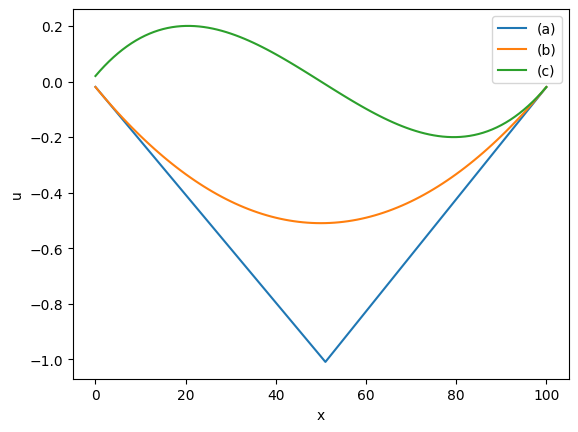
\includegraphics[scale=0.45]{./img/resultado_tridiag}}
\caption{Resultado de las funciones}
\label{result_laplaciano}
\end{figure}

Analizando con mayor profundidad cada función:\par
\begin{enumerate}
    \item[a)] La derivada segunda de la función (a) es 0 para todo x distinto a $i = n/2 + 1$. Luego, la derivada primera de la función (a) es constante para todo x $\not =$ i,lo que implica que la función es lineal para todo x $\not =$ i. Por lo que i es un punto de inflexión. Como la derivada segunda en i es positiva, la función tiene que ser cóncava para los positivos. Esta función descripta es coherente con la figura graficada.

    \item[b)] La derivada segunda de la función (b) es $\frac{4}{n^2}$ para todo x. Entonces, la derivada primera es lineal para todo x, lo que implica que la función es cuadrática para todo x. La función graficada se corresponde con una cuadrática.

    \item[c)] La derivada segunda de la función (c) es una función lineal para todo x. Esto significa que la derivada primera es cuadrática, implicando que la función debe ser un polinomio de grado tres (cúbica). La función graficada se corresponde con una cúbica.
\end{enumerate}



\subsection{Tiempos de cómputo}
Como explicamos anteriormente, los diferentes algoritmos tienen complejidades computacionales muy distintas, lo que afecta significativamente el tiempo de ejecución y los recursos necesarios para resolver un problema.

En el caso de la eliminación gaussiana, el algoritmo con pivoteo tiene una complejidad cúbica ($\mathcal{O}$(n$^3$)), lo que significa que el tiempo de ejecución crece rápidamente a medida que aumenta el tamaño de la matriz. Por otro lado, los algoritmos diseñados específicamente para matrices con estructura especial, como el caso de las matrices tridiagonales, pueden reducir esa complejidad a $\mathcal{O}$(n), lo que implica una mejora considerable en términos de rendimiento.Por lo tanto, Lo esperado es que el algoritmo tridiagonal sea notablemente más rápido a comparación del algoritmo de eliminación gaussiana con pivoteo

Para evaluar el rendimiento de los distintos algoritmos de eliminación gaussiana, se generaron matrices y vectores correspondientes a cada tamaño seleccionado. Posteriormente, se implementaron los algoritmos de eliminación gaussiana con pivoteo, eliminación gaussiana para matrices tridiagonales, tanto en su versión estándar como en la versión con precomputo, para dimensiones que corresponden a potencias de dos (2$^k$). Este proceso fue repetido 10 veces, registrando el tiempo mínimo de ejecución en cada iteración. Esta repetición busca mitigar el posible efecto de las variaciones causadas por la organización del computador (posición de las variables en memoria por ejemplo).

Considerando, las complejidades temporales teóricas de los algoritmos:

\begin{itemize}
    \item Eliminación Gaussiana con pivoteo: $O(n^{3})$
    \item Eliminación Gaussiana para matrices tridiagonales estándar: $O(n)$
    \item Eliminación Gaussiana para matrices tridiagonales con precomputo: $O(n)$
\end{itemize}


Definimos \textit{A} como la matriz Laplaciana, es decir, aquella matriz que tiene a -2 como elementos de la diagonal y a 1 como los elementos de las dos subdiagonales. Obtenemos el siguiente resultado (figura \ref{result_ej5})

\begin{figure}[H]
\centerline{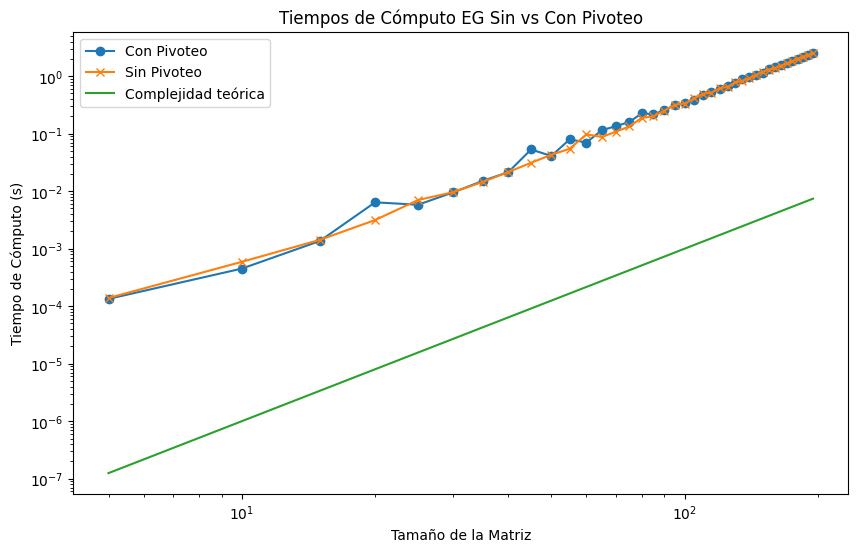
\includegraphics[scale=0.45]{./img/tiempos_EGsinVsConPivoteo.png}}
\caption{Tiempo de computo para EG con pivoteo y EG en un sistema tridiagonal}
\label{result_ej5}
\end{figure}

Como era esperado, como los algoritmos de las matrices tridiagonales trabajan a nivel vectorial, modificando los valores de los vectores b y c, la complejidad temporal mejora.

%Los resultados obtenidos se pueden ver en la sección \ref{resultados}


\subsection{Simulación de difusión}

Para expresar la ecuación de difusión se considera el incremento para el paso \textit{k}, $u^k - u^{k-1}$ como una
fracción ($\alpha$) del operador laplaciano aplicado a $u^{k-1}$ (ecuación explícita) y a $u^{k}$ (ecuación implícita):
\begin{center}
  $u_i^{(k)} - u_i^{(k-1)}$ = $\alpha(u_{i-1}^{(k-1)} - 2u_i^{(k-1)} + u_{i+1}^{(k-1)}) - Eq (3)$
\end{center}

\begin{center}
  $u_i^{(k)} - u_i^{(k-1)}$ = $\alpha(u_{i-1}^{(k)} - 2u_i^{(k)} + u_{i+1}^{(k)}) - Eq (4)$
\end{center}

Reordenando los términos, obtenemos una solución de forma explícita para la ecuación (3). Ésta responde a la forma $u^{(k)} = A \times u^{(k-1)}$. Por otro lado, reordenando los términos de la ecuación (4) obtenemos una solución de forma implícita: A$\times u^{(k)}$ = $u^{(k-1)}$. De esta forma, para obtener la evolución, resolvemos el sistema de ecuaciones para cada paso $k$.
Utilizando la última formulación, logramos generar soluciones estables para todos los valores.

Para la solución implícita podemos notar que se genera un sistema tridiagonal, lo que nos permite utilizar el algoritmo de eliminación Gaussiana para sistemas tridiagonales. La eliminación Gaussiana no requiere pivoteo por la estructura de la matriz de derivada segunda. La triangulación finaliza en una matriz donde los elementos de la diagonal principal son: $a_{ii} = - \frac{i+1}{i}$. 
Es así que, como en ningún paso queda un elemento de la diagonal igual a cero, no se requiere pivoteo.\par
Los resultados se discutirán en la sección \ref{resultados}, teniendo en cuenta que los parámetros utilizados fueron n = 101, r = 10, m = 1000.


\subsubsection{Simulación de difusión 2D}
 El objetivo es implementar una simulación de cómo se difunde el calor en una placa de 15x15 unidades. El calor se origina en un punto central con una temperatura fija de 100 unidades, mientras que los bordes de la placa se mantienen siempre a 0. Este tipo de simulaciones se basa en la ecuación de difusión, que modela cómo el calor se dispersa en el tiempo.
 Para esto utilizaremos el método implícito, lo que implica que cada paso de tiempo requiere resolver un sistema de ecuaciones lineales. Esto nos garantiza estabilidad, incluso si el coeficiente de difusión $\alpha$ = 0.1 varía.
Por otro lado, a diferencia de la simulación anterior la matriz resultante en 2D no será tridiagonal, sino pentadiagonal, debido a que cada punto de la placa interactúa con sus vecinos en las cuatro direcciones.
En la sección \ref{resultados} visualizaremos cómo cambia la distribución de temperatura en la placa a medida que pasa el tiempo.

